\chapter{Resultados}

Neste capítulo serão apresentados os resultados preliminares, provenientes dos testes realizados bem como refinamento da ferramenta e seus parâmetros. A seção 4.1 apresentará os resultados obtidos com o \textit{PhotoGuide}; na seção 4.2 os resultados preliminares com o \textit{LSD-SLAM} serão mostrados. A seção 4.3 trará os problemas encontrados.

\section{Resultados com o \textit{PhotoGuide}}

Primeiramente o aplicativo operou sem usar nenhuma das três formas de filtragem descritas anteriormente, ocasionando num grande número de falsos casamentos, como apresentam as imagens \ref{fig4:1} e \ref{fig4:2}:

\begin{figure}[H]
	\centering
		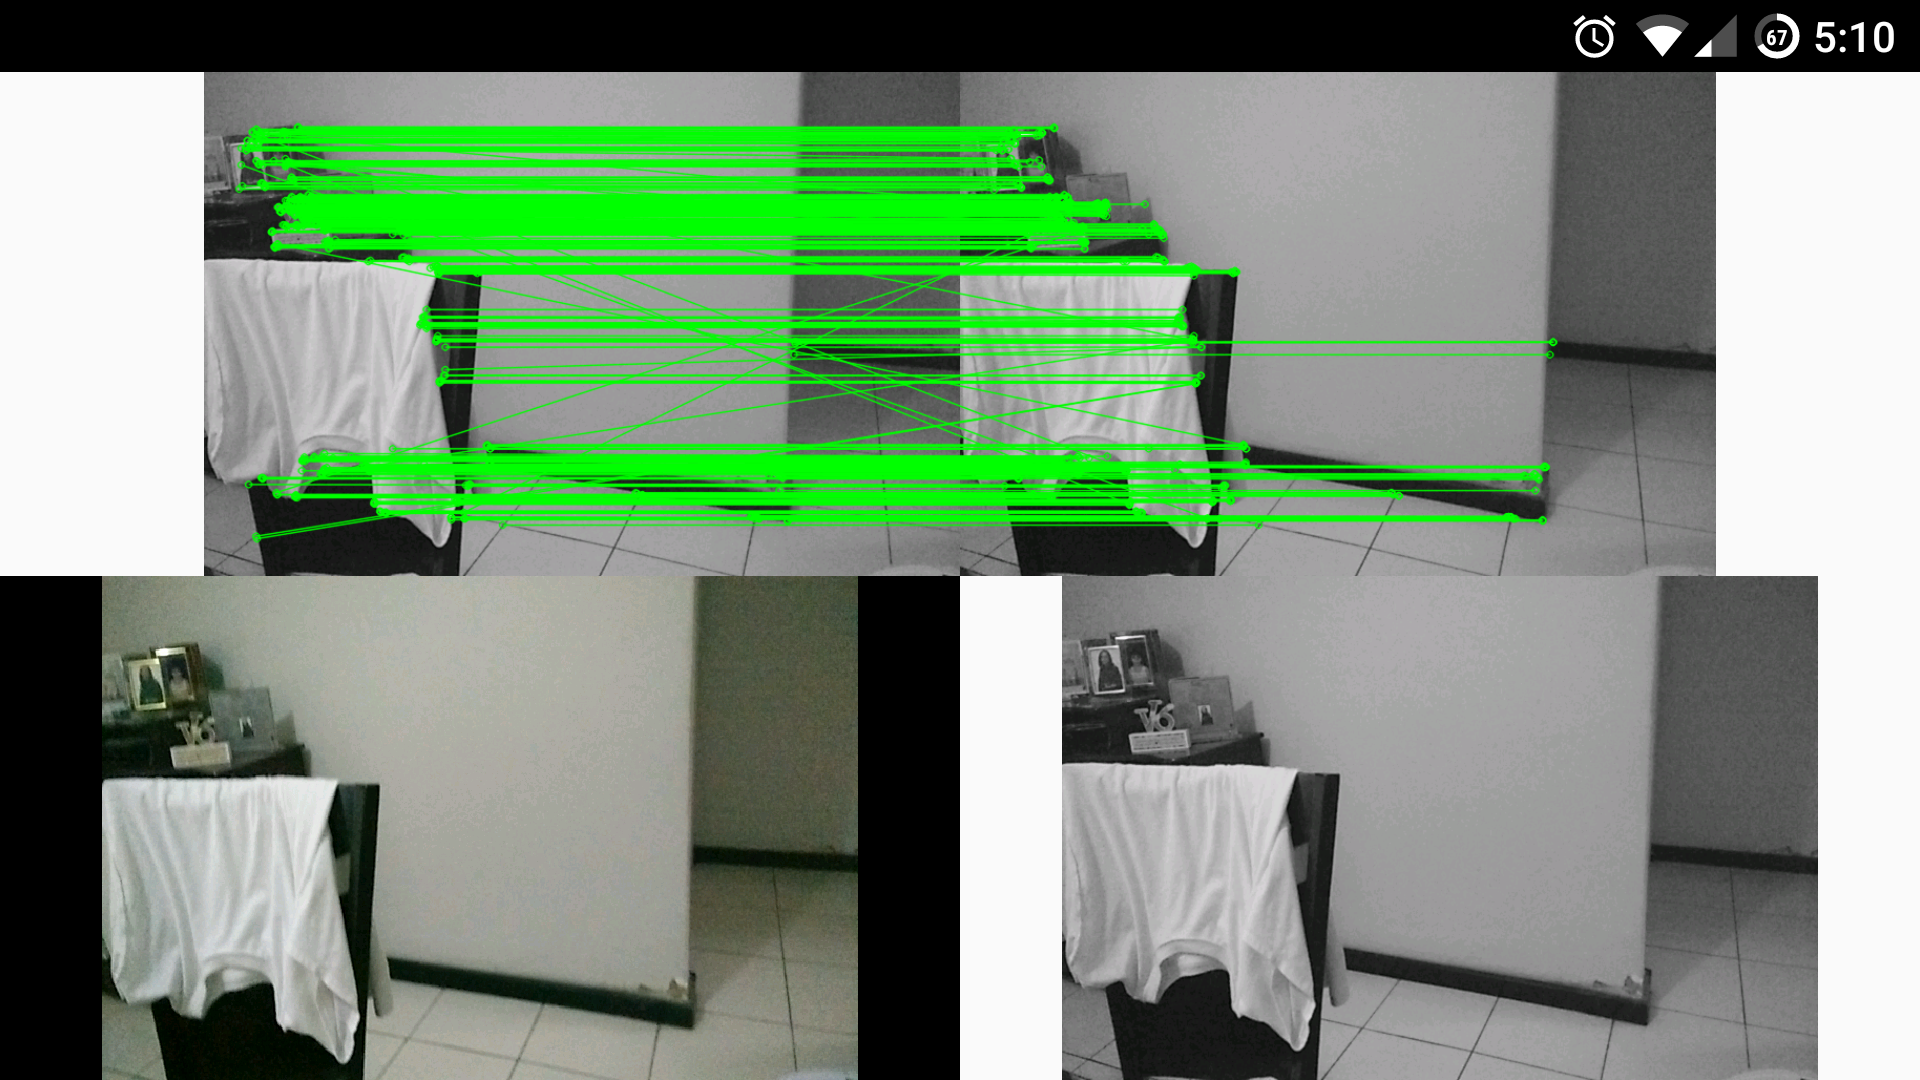
\includegraphics[width= \textwidth]{Imagens/figura4-1.png}
	\caption{Exemplo de execução do \textit{PhotoGuide} sem nenhuma filtragem de casamentos}
	\label{fig4:1}
\end{figure}

\begin{figure}[H]
	\centering
		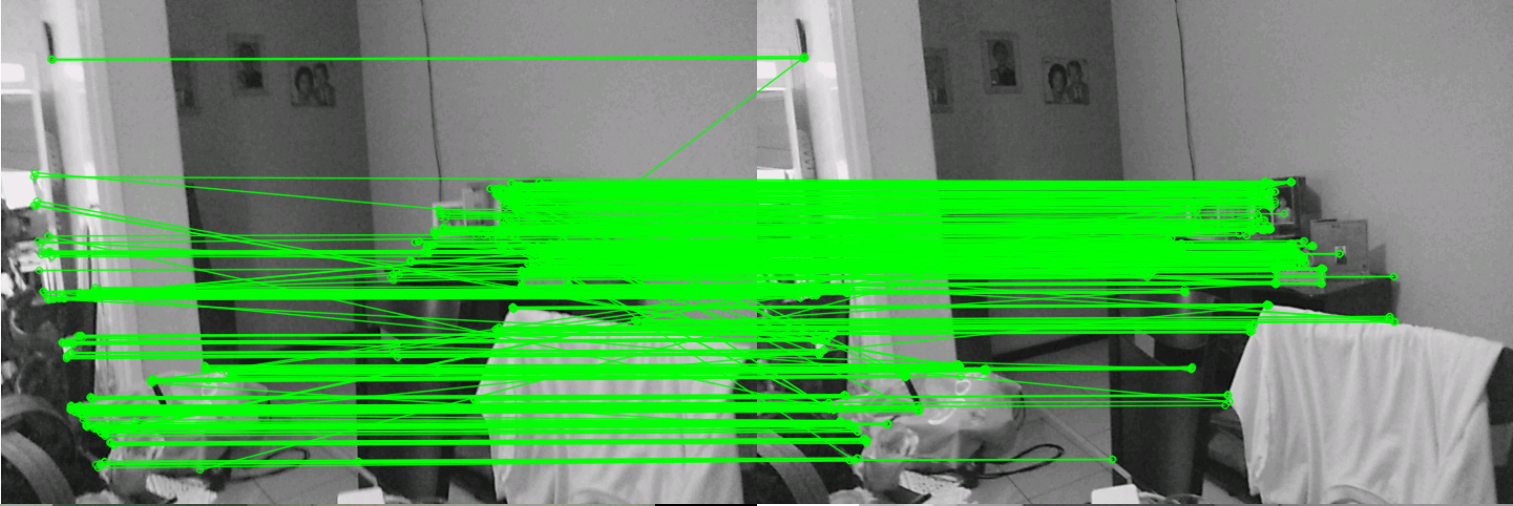
\includegraphics[width= \textwidth]{Imagens/figura4-2.png}
	\caption{Segundo exemplo de execução do \textit{PhotoGuide} sem nenhuma filtragem de casamentos}
	\label{fig4:2}
\end{figure}

Essa situação é pior quando o ambiente possui partes em vidro, como mesas ou janelas, dificultando ainda mais a casamento de pontos, como mostra a Figura \ref{fig4:3}

\begin{figure}[H]
	\centering
		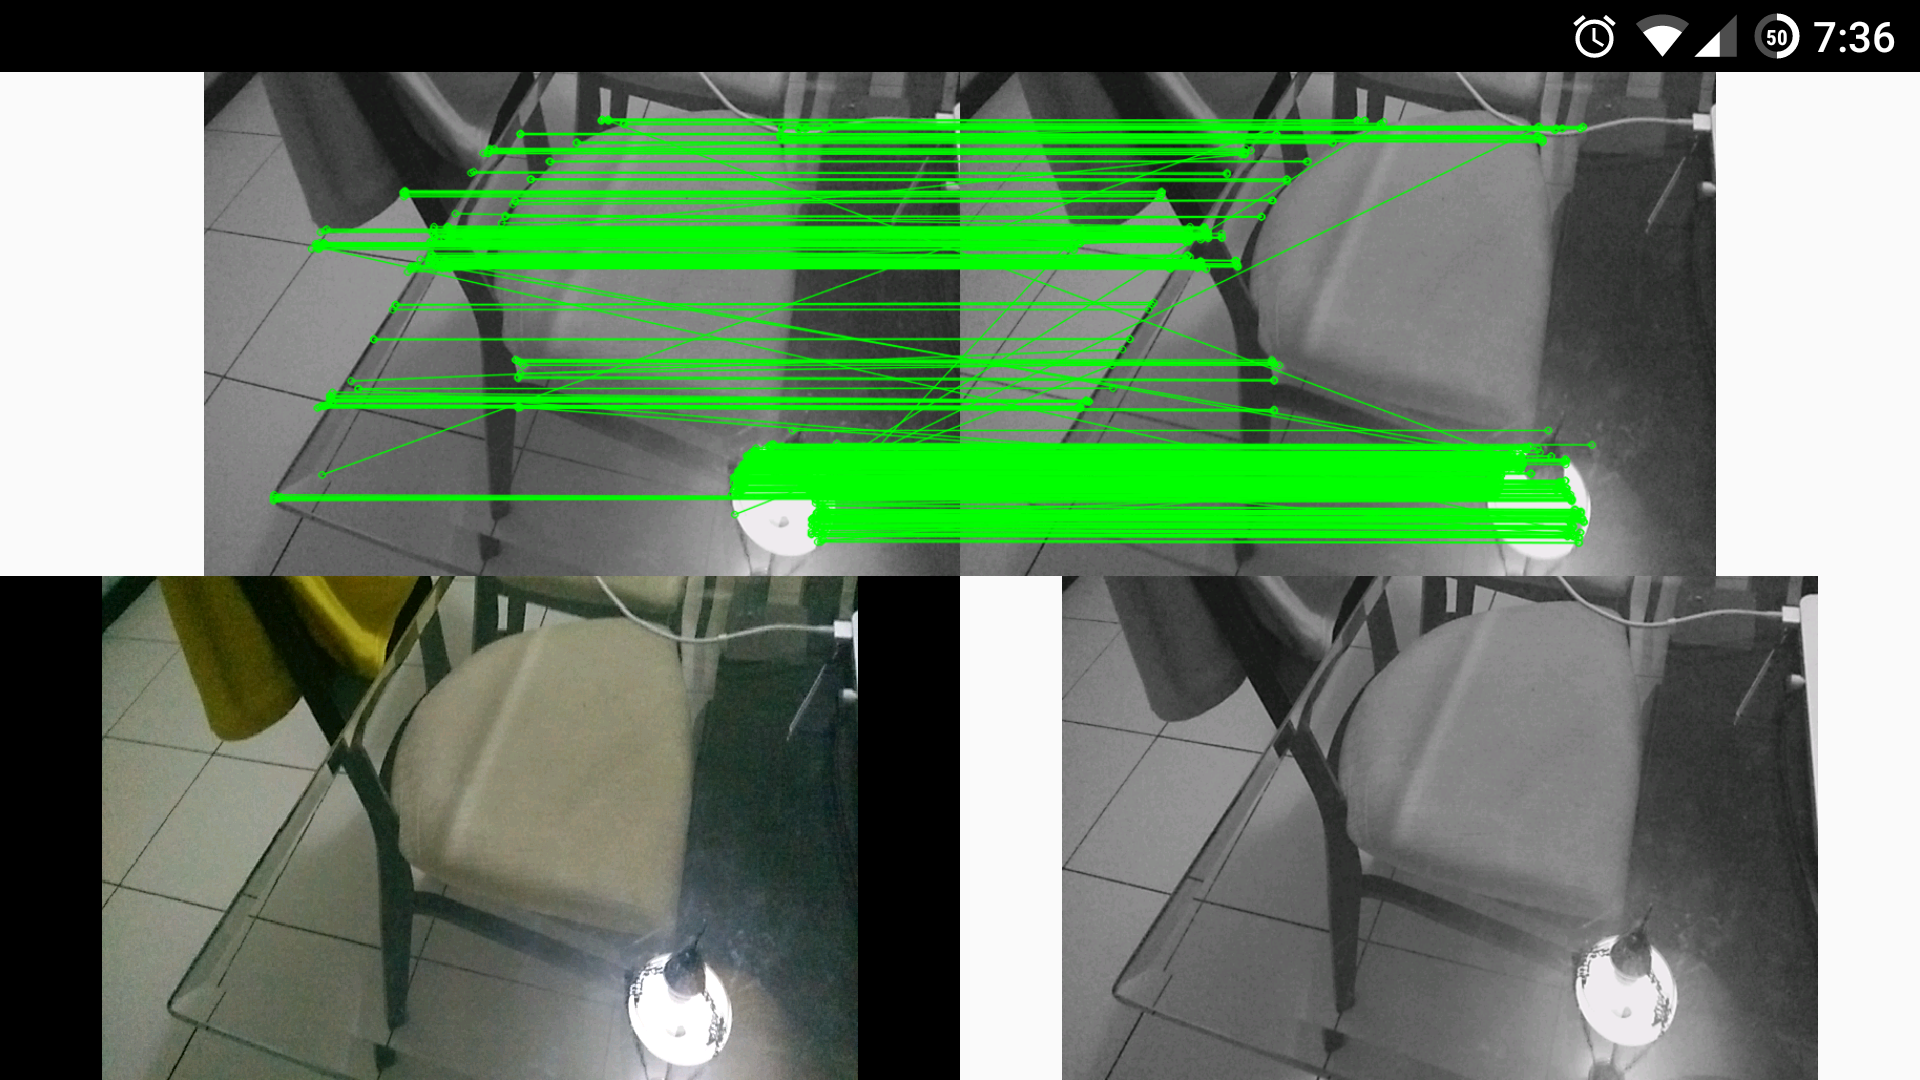
\includegraphics[width= \textwidth]{Imagens/figura4-3.png}
	\caption{Exemplo de execução do \textit{PhotoGuide} sem nenhuma filtragem de casamentos e com peças em vidro, dificultando os casamentos}
	\label{fig4:3}
\end{figure}

Ao se adicionar os métodos de filtragem explicados na seção 3.1, é possível eliminar diversos casamentos errôneos, como na Figura \ref{fig4:4}:

\begin{figure}[H]
	\centering
		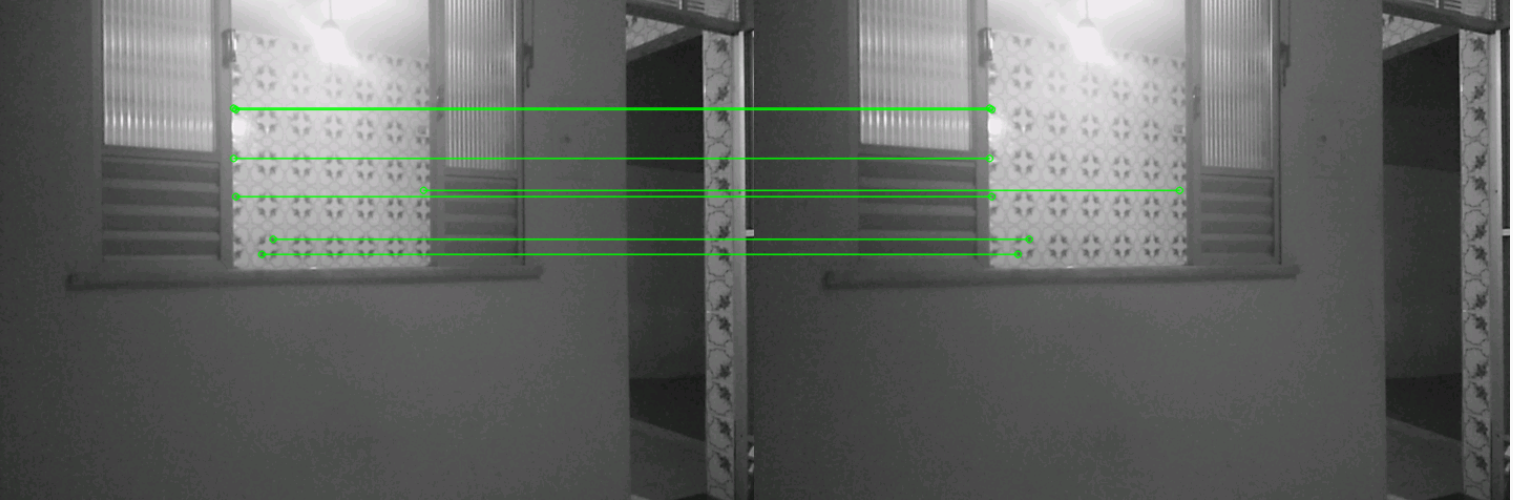
\includegraphics[width= \textwidth]{Imagens/figura3-2E4-4.png}
	\caption{Exemplo da filtragem de casamentos}
	\label{fig4:4}
\end{figure}

Infelizmente, dependendo do ambiente, o número de casamentos pode ser muito pequeno para se tornar significativo para a reconstrução 3D. Foram realizados testes diminuindo a sensibilidade com qual os casamentos eram filtrados, ou a não execução de alguma filtragem, mas ainda eram encontrados falso positivos, sendo necessário todos os métodos de filtragem. 
	Tendo em vista os problemas com o desempenho no aparelho utilizado, bem como problemas com o algoritmo, a continuação do trabalho se deu com a ferramenta \textit{LSD-SLAM}, e a funcionalidade de calibração e exportação de arquivo de calibração do \textit{PhotoGuide} foi útil para utilizar a calibração de \textit{smartphones} em testes com o \textit{LSD-SLAM}, bem como a possibilidade de trabalhos futuros onde seja desejável a exportação da calibração da câmera ou obter \textit{dataset} usando o \textit{smartphone}.
	
\section{Resultados com o \textit{LSD-SLAM}}

O \textit{LSD-SLAM} possui diversos parâmetros que podem auxiliar na visualização e refinamento de como seus algoritmos funcionam. Os testes foram realizados em um dos laboratórios do DCOMP, mais precisamente, o laboratório de mestrado II, na área externa do prédio e também em um quintal, este último para testar os resultados sob um ambiente com mais texturas e menos homogêneo. As Figuras \ref{fig4:5} a \ref{fig4:15} mostram as \textit{PointClouds} obtidas e fotografias dos ambientes:

\begin{figure}[H]
	\centering
		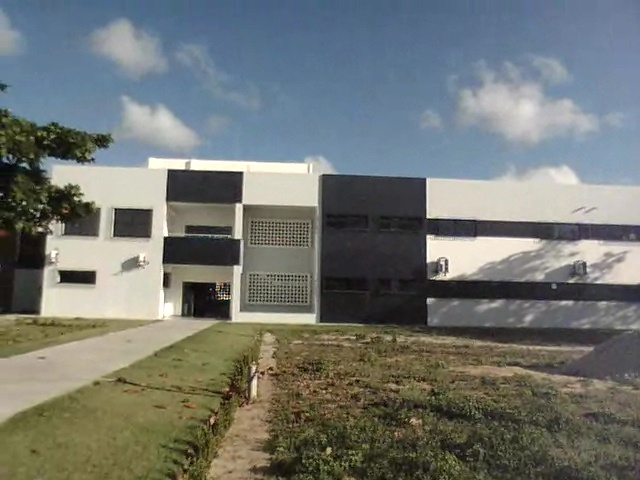
\includegraphics[width= \textwidth]{Imagens/figura4-7.jpg}
	\caption{Fotografia da área externa do DCOMP}
	\label{fig4:7}
\end{figure}

\begin{figure}[H]
	\centering
		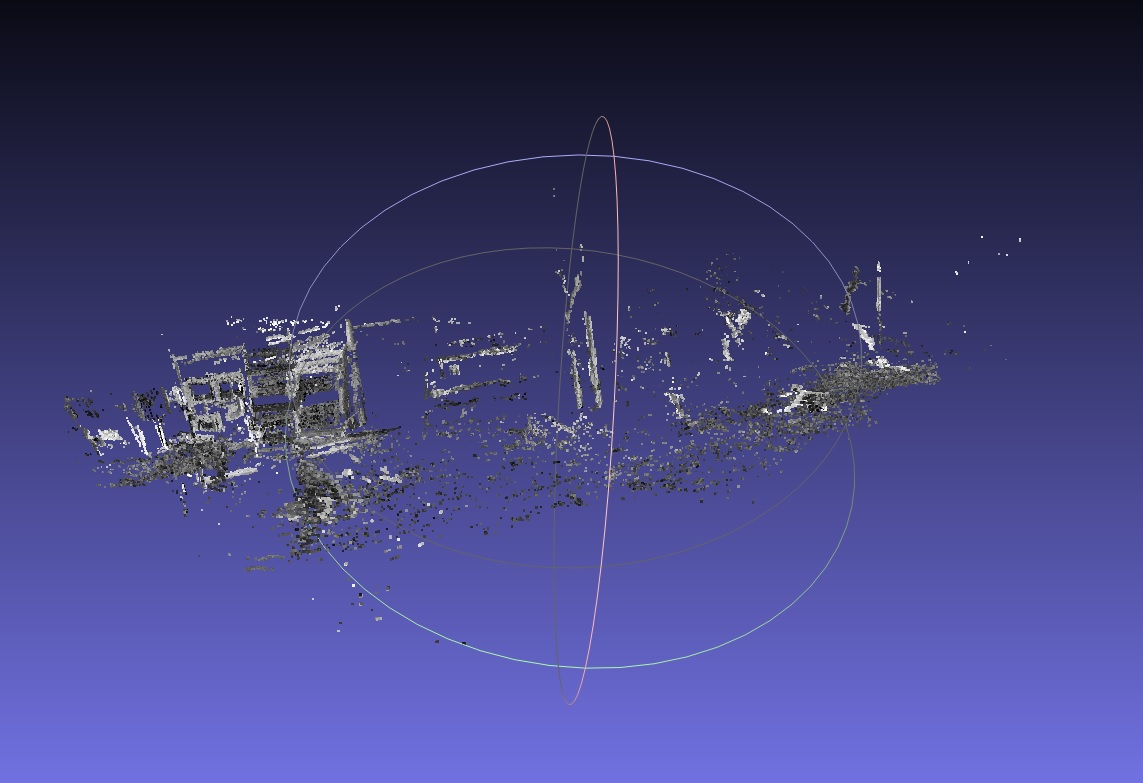
\includegraphics[width= \textwidth]{Imagens/figura4-5.jpg}
	\caption{\textit{Nuvem de pontos} da área externa do DCOMP com a câmera \textit{PSEye®} com 119621 pontos (a)}
	\label{fig4:5}
\end{figure}

\begin{figure}[H]
	\centering
		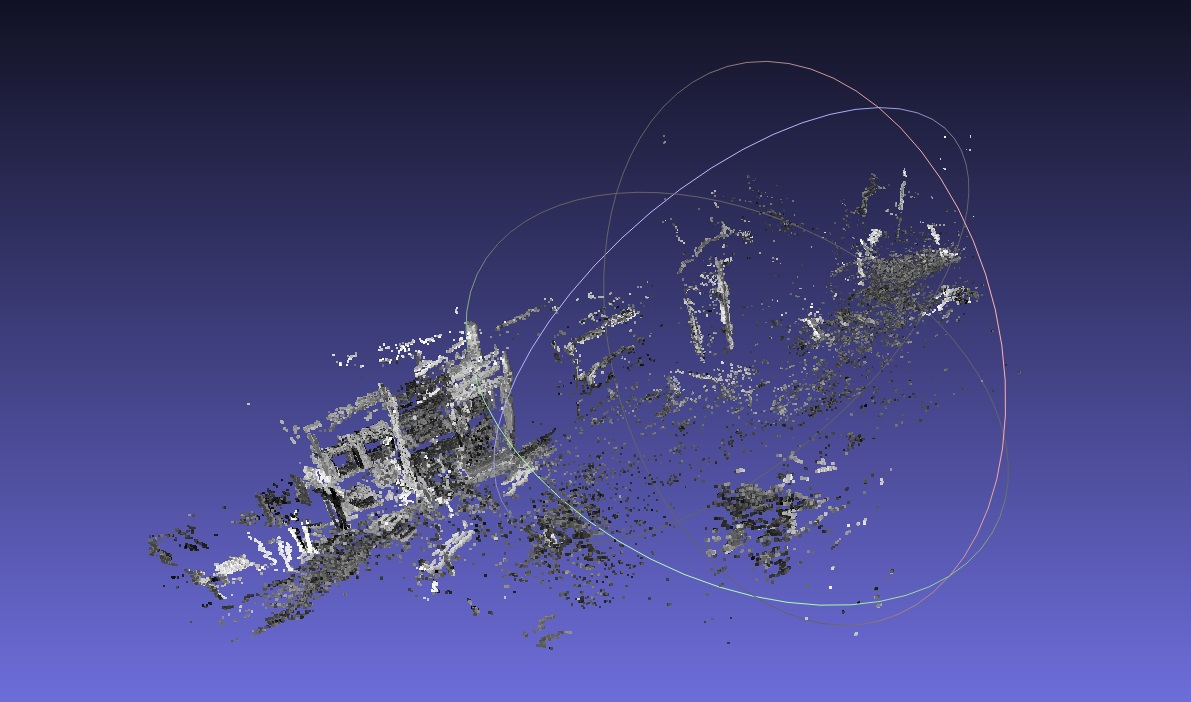
\includegraphics[width= \textwidth]{Imagens/figura4-6.jpg}
	\caption{\textit{Nuvem de pontos} da área externa do DCOMP com a câmera \textit{PSEye®} com 119621 pontos (b)}
	\label{fig4:6}
\end{figure}


\begin{figure}[H]
	\centering
		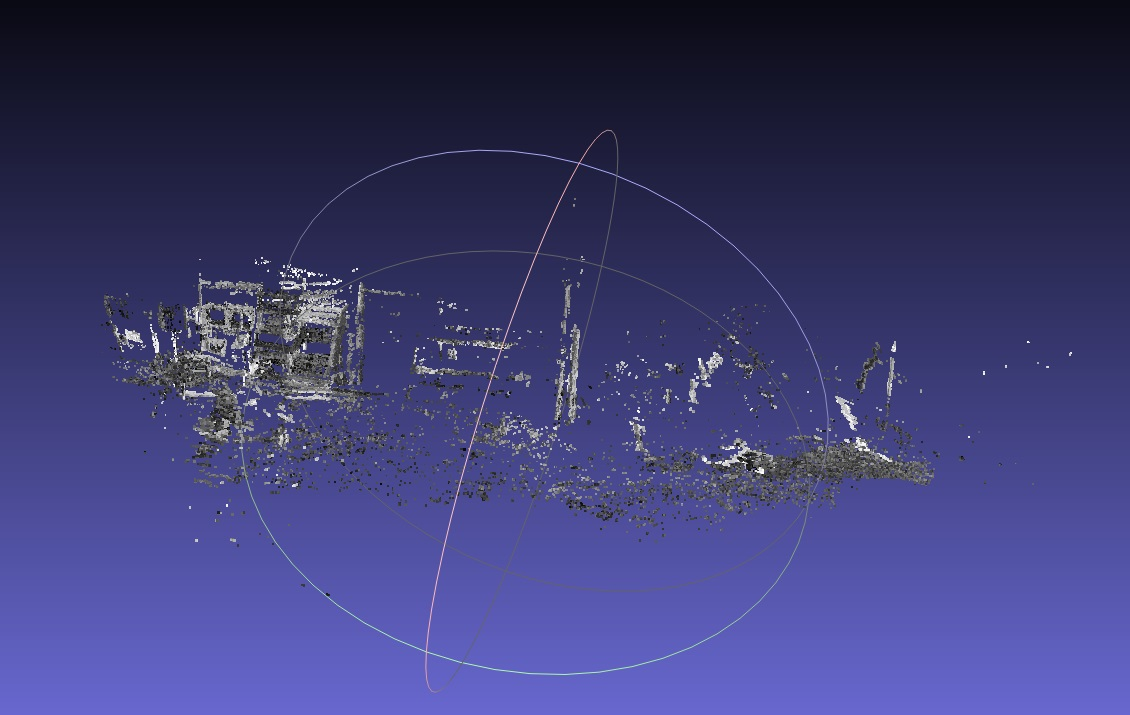
\includegraphics[width= \textwidth]{Imagens/figura4-8.jpg}
	\caption{Outra \textit{nuvem de pontos} da área externa do DCOMP usando a \textit{PSEye®} com 119621 pontos , sob outro ângulo}
	\label{fig4:8}
\end{figure}

\begin{figure}[H]
	\centering
		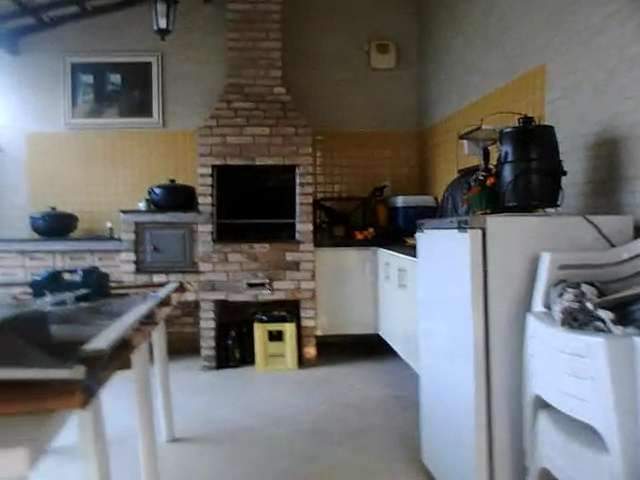
\includegraphics[width= \textwidth]{Imagens/figura4-12.jpg}
	\caption{Fotografia do quintal}
	\label{fig4:12}
\end{figure}

\begin{figure}[H]
	\centering
		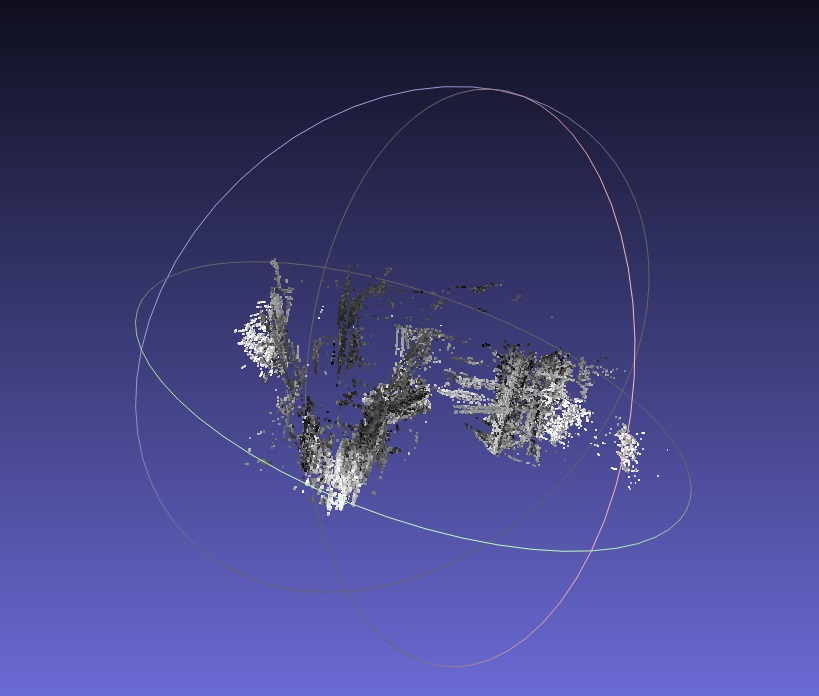
\includegraphics[width= \textwidth]{Imagens/figura4-10.jpg}
	\caption{\textit{Nuvem de pontos} do quintal de uma casa com 87093 pontos (a)}
	\label{fig4:10}
\end{figure}

\begin{figure}[H]
	\centering
		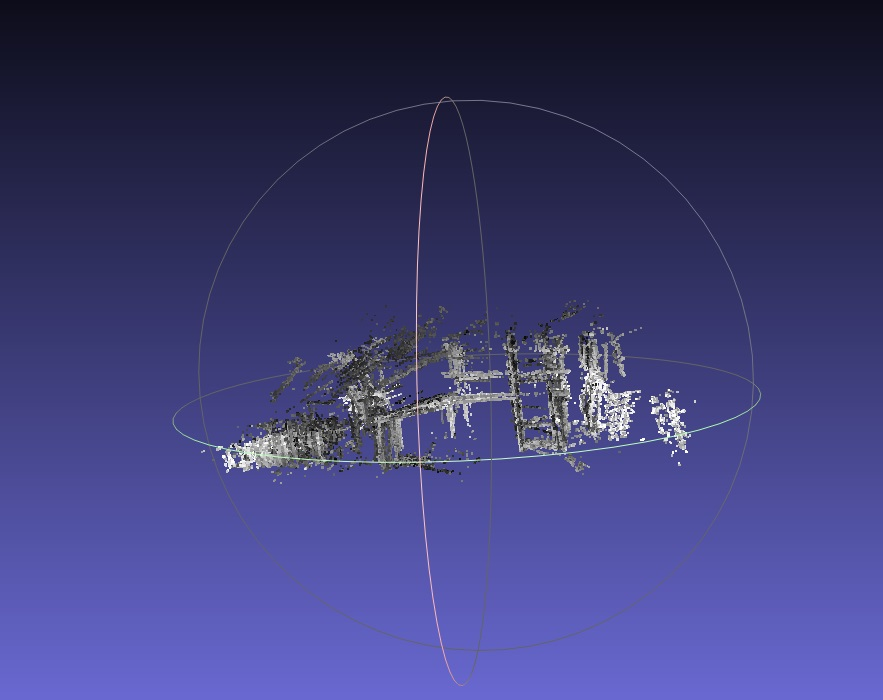
\includegraphics[width= \textwidth]{Imagens/figura4-11.jpg}
	\caption{\textit{Nuvem de pontos} do quintal de uma casa com 87093 pontos (b)}
	\label{fig4:11}
\end{figure}

\begin{figure}[H]
	\centering
		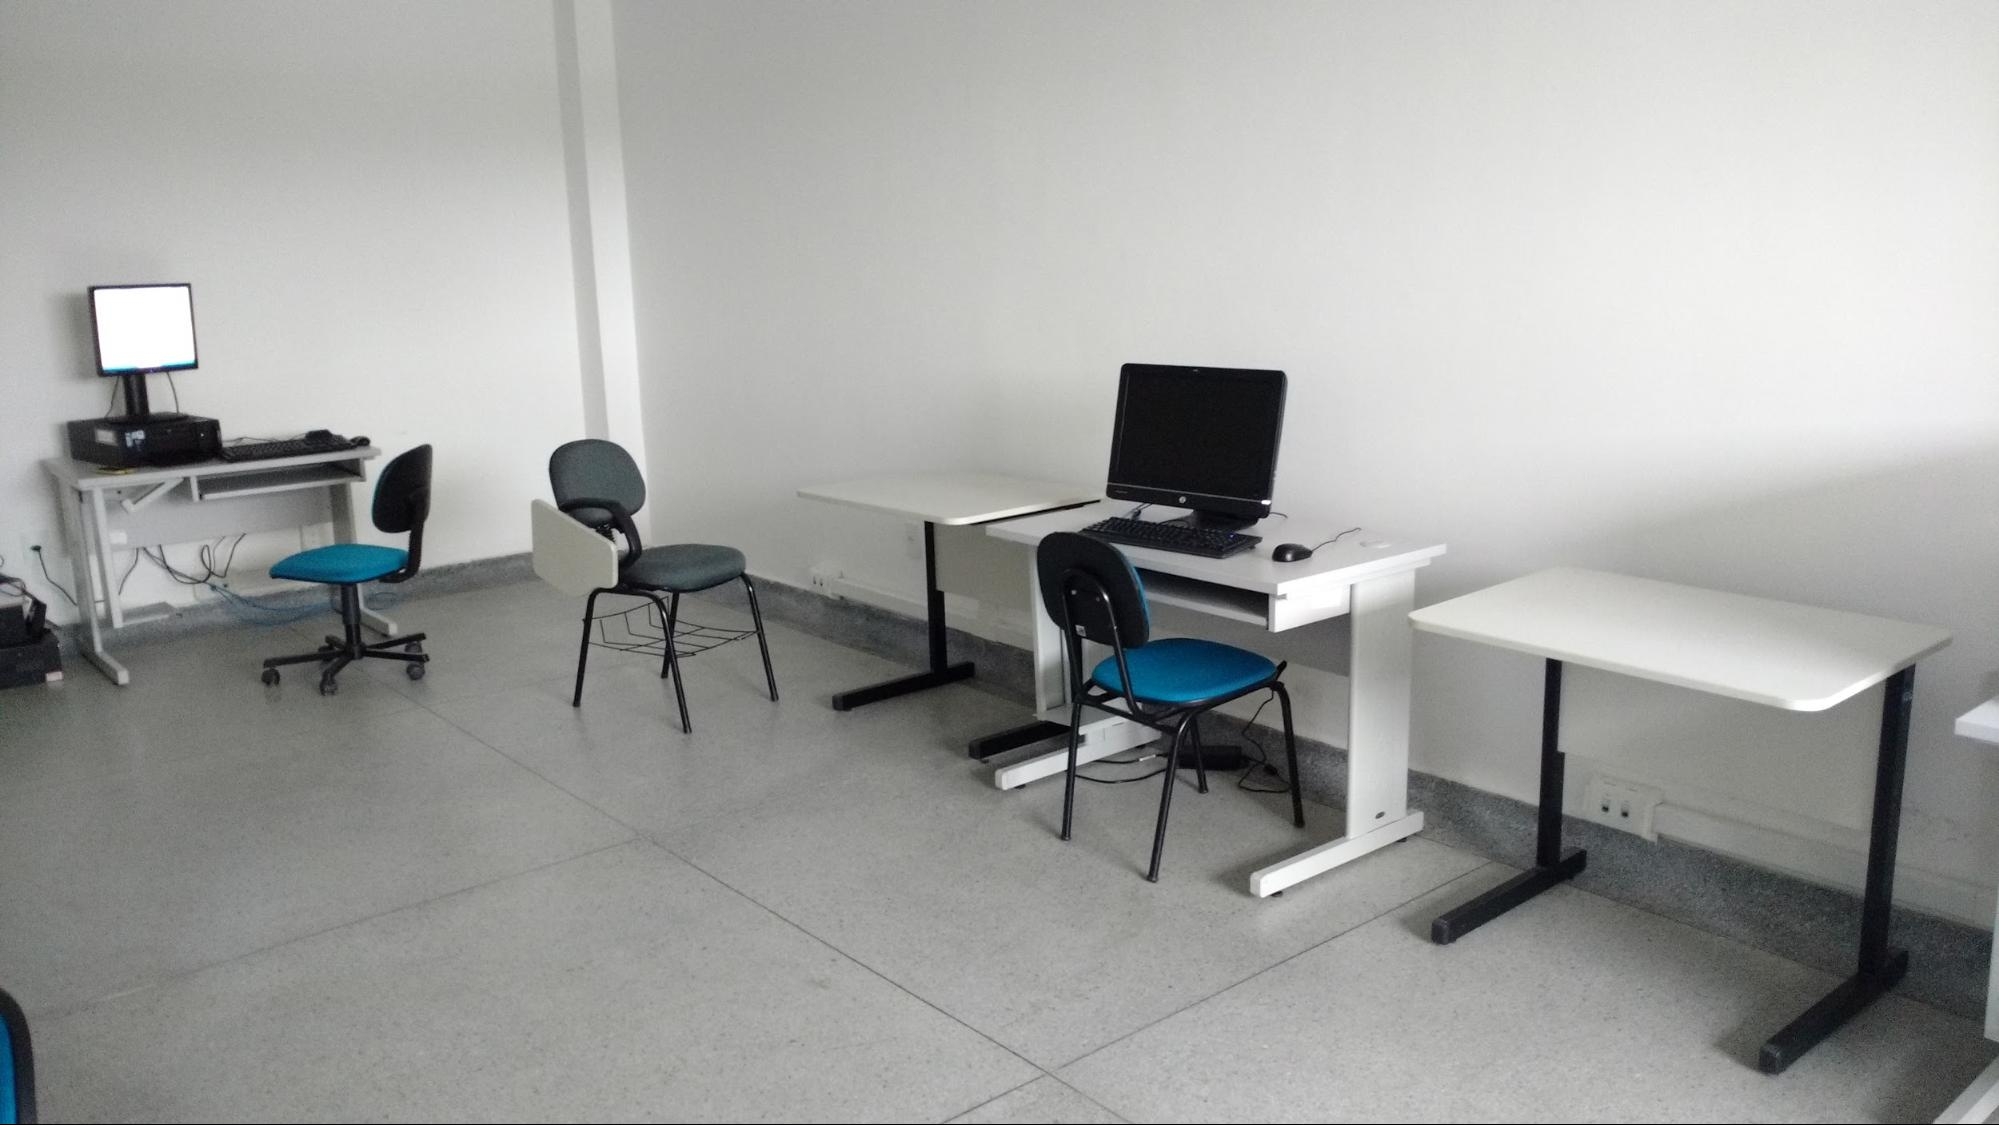
\includegraphics[width= \textwidth]{Imagens/figura4-15.jpg}
	\caption{Fotografia do laboratório de mestrado II}
	\label{fig4:15}
\end{figure}

\begin{figure}[H]
	\centering
		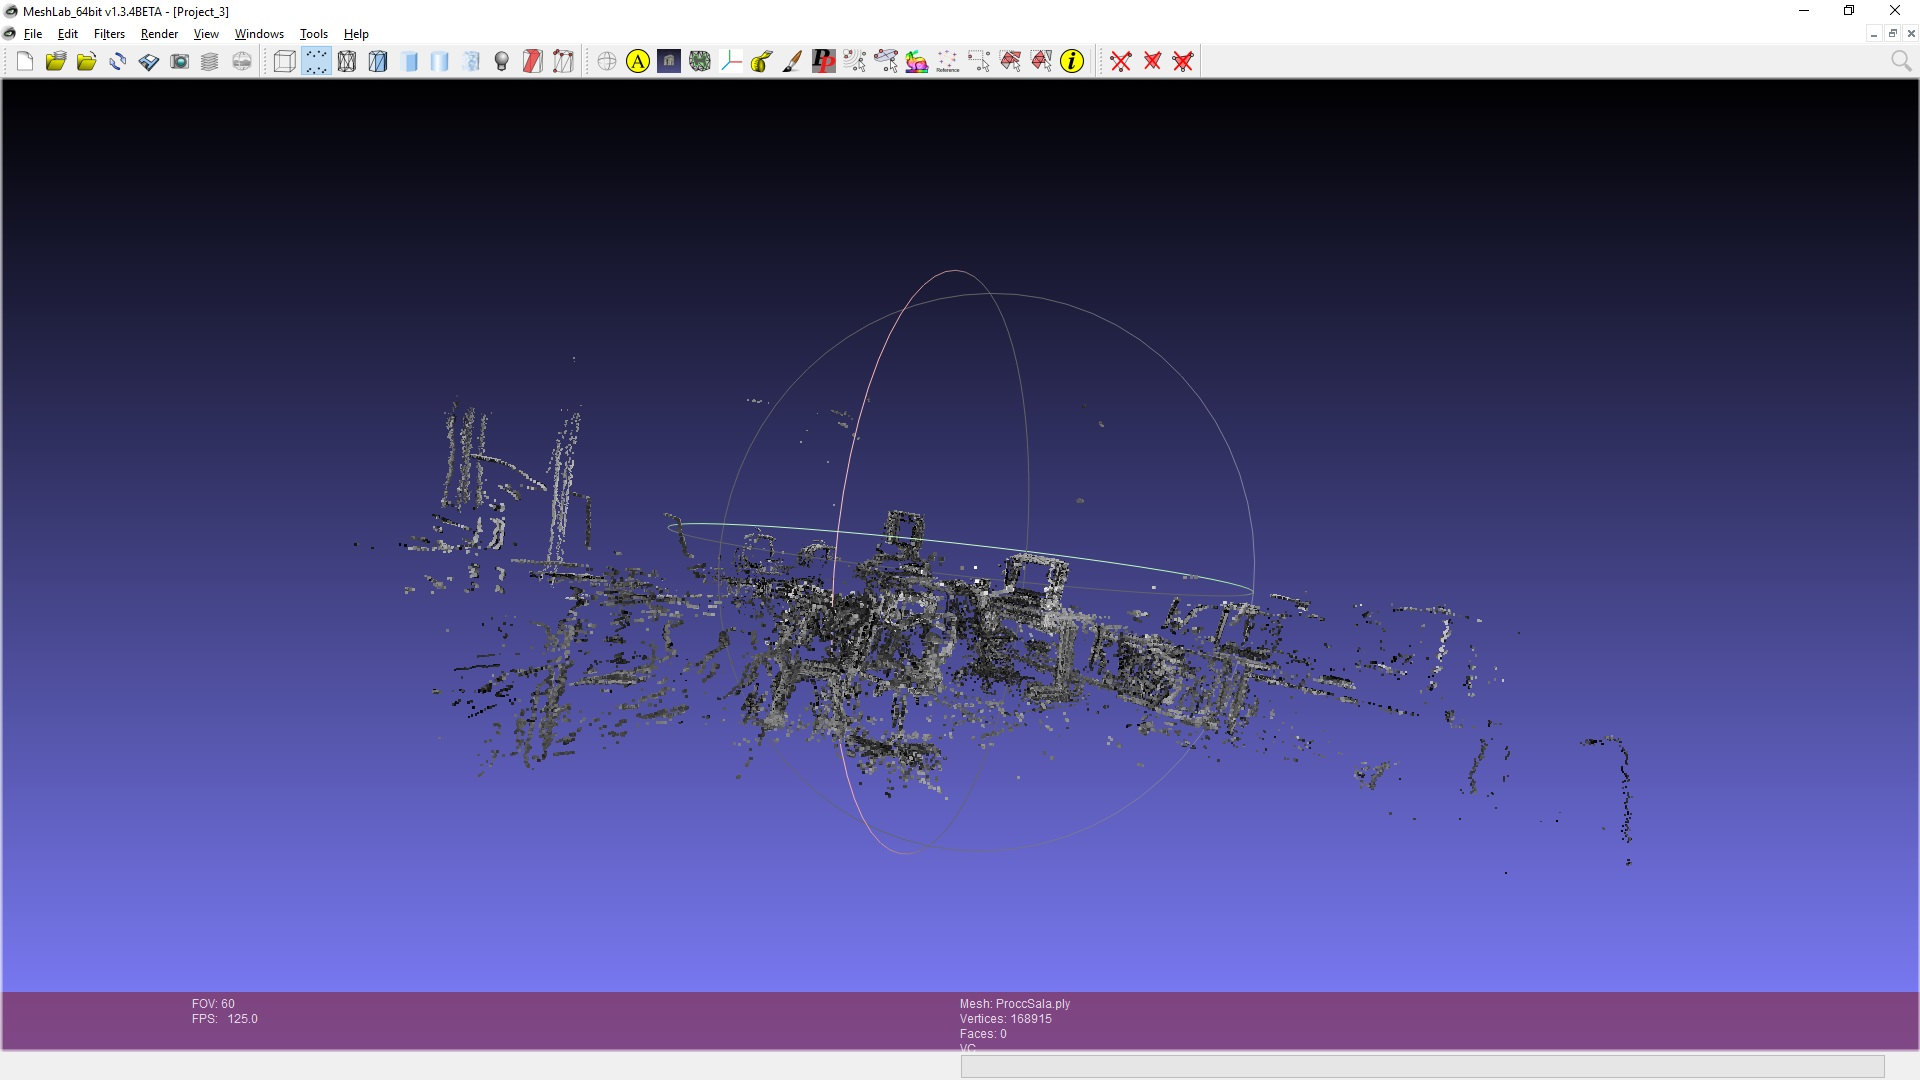
\includegraphics[width= \textwidth]{Imagens/figura4-13.jpg}
	\caption{\textit{Nuvem de pontos} do laboratório de mestrado II com 168915 pontos (a)}
	\label{fig4:13}
\end{figure}

\begin{figure}[H]
	\centering
		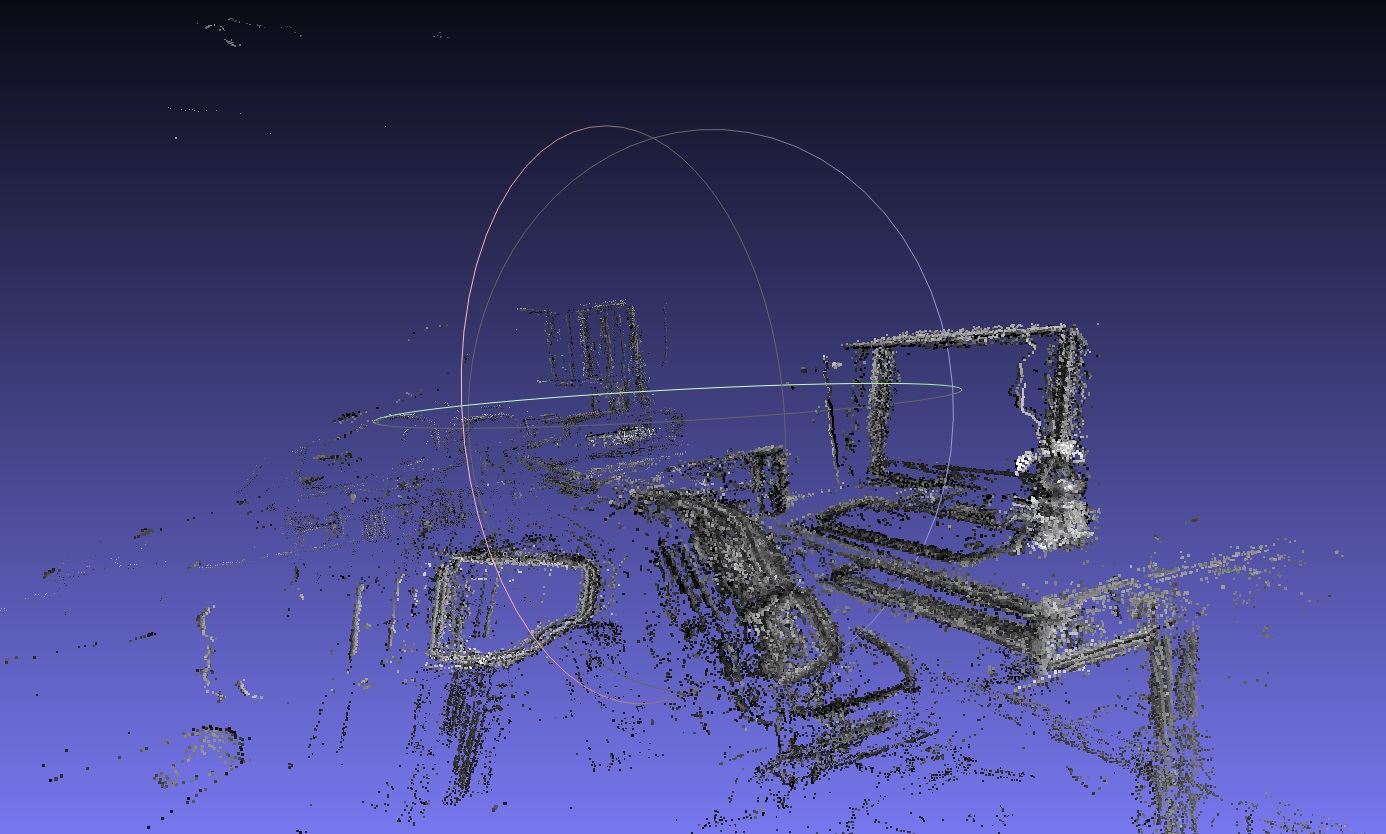
\includegraphics[width= \textwidth]{Imagens/figura4-14.jpg}
	\caption{\textit{Nuvem de pontos} do laboratório de mestrado II com 168915 pontos (b)}
	\label{fig4:14}
\end{figure}

\begin{figure}[H]
	\centering
		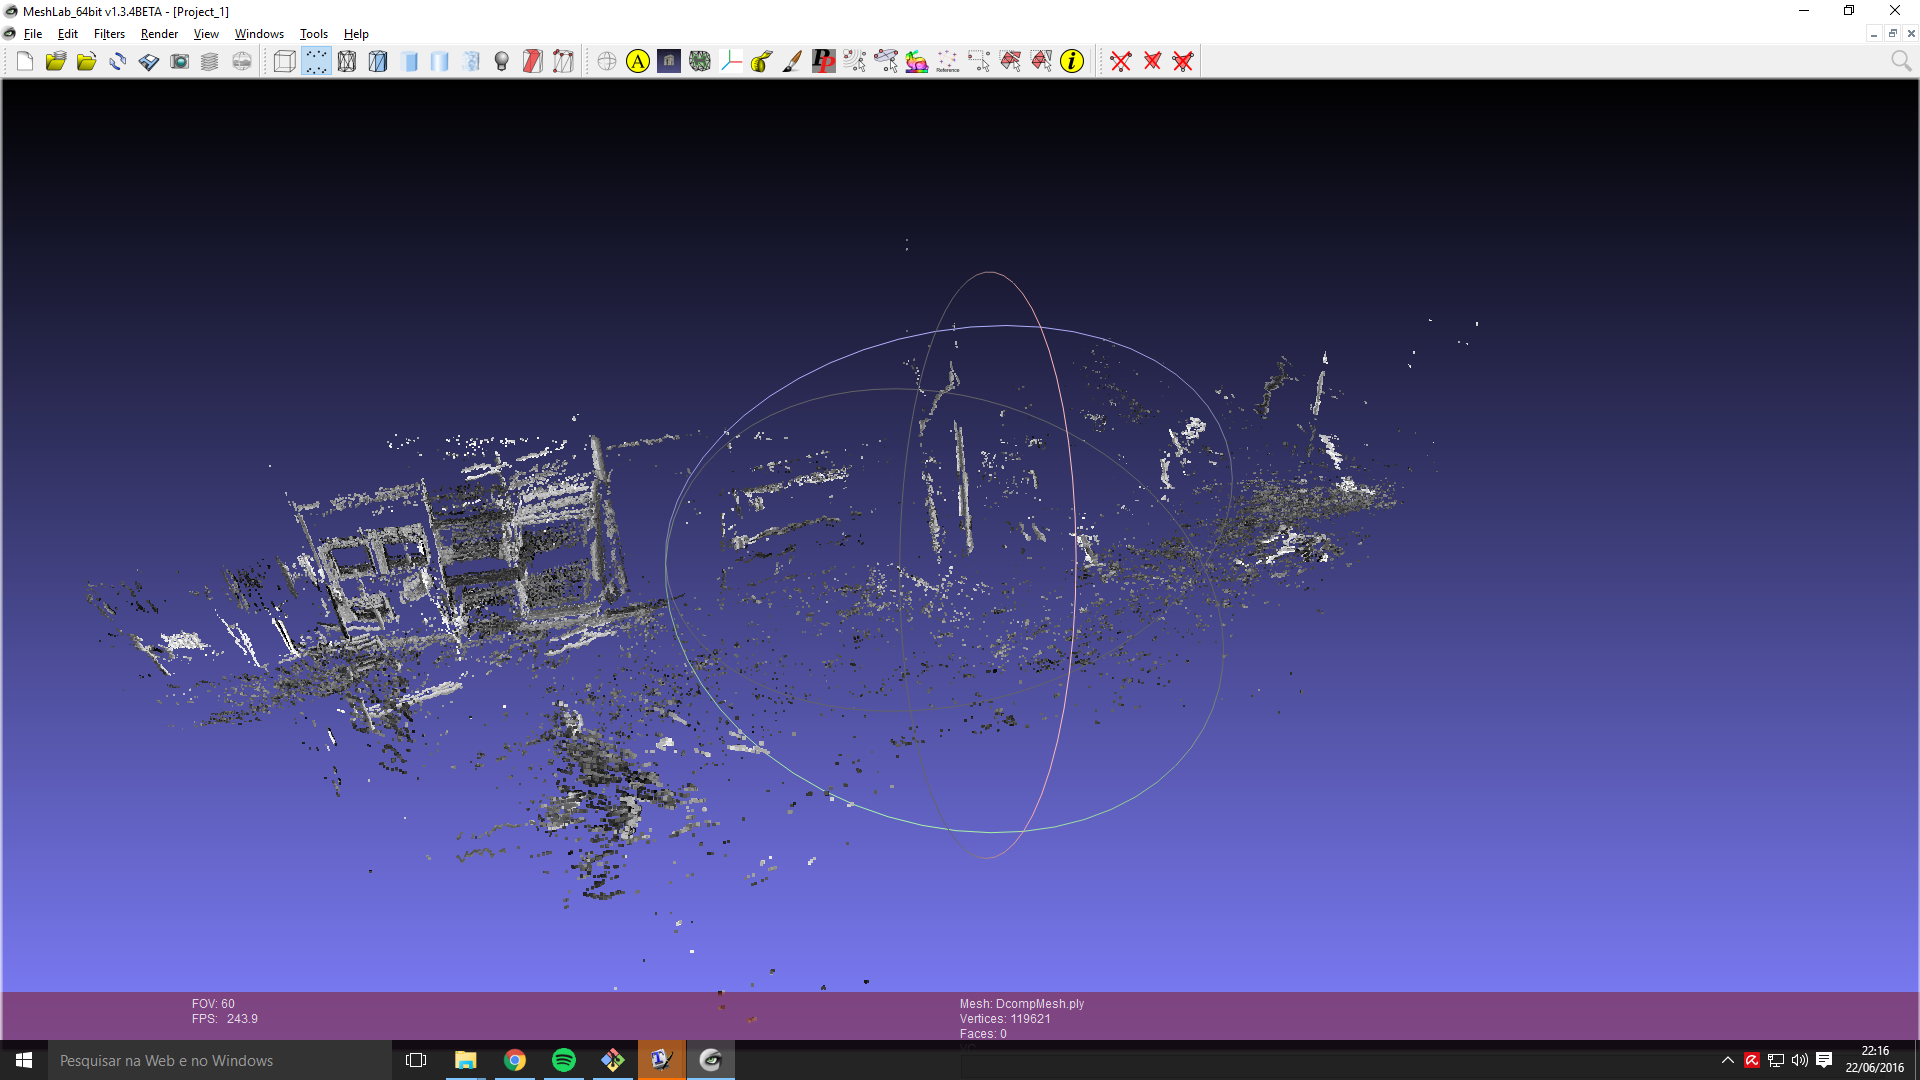
\includegraphics[width= \textwidth]{Imagens/dcompMotox.PNG}
	\caption{\textit{Nuvem de pontos} da área externa do DCOMP usando a câmera do \textit{smartphone Motorola® Moto X Play} com 3680087 pontos}
\end{figure}

\begin{figure}[H]
	\centering
		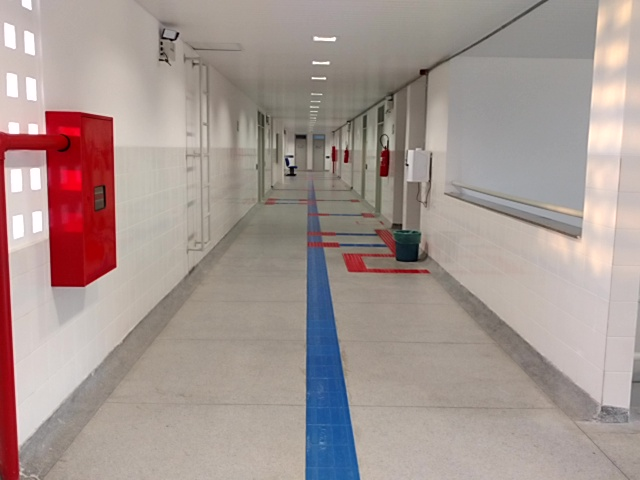
\includegraphics[width= \textwidth]{Imagens/scene00087.jpg}
	\caption{Fotografia do DCOMP usando a câmera do \textit{smartphone Motorola® Moto X Play} com 3680087 pontos}
\end{figure}

\begin{figure}[H]
	\centering
		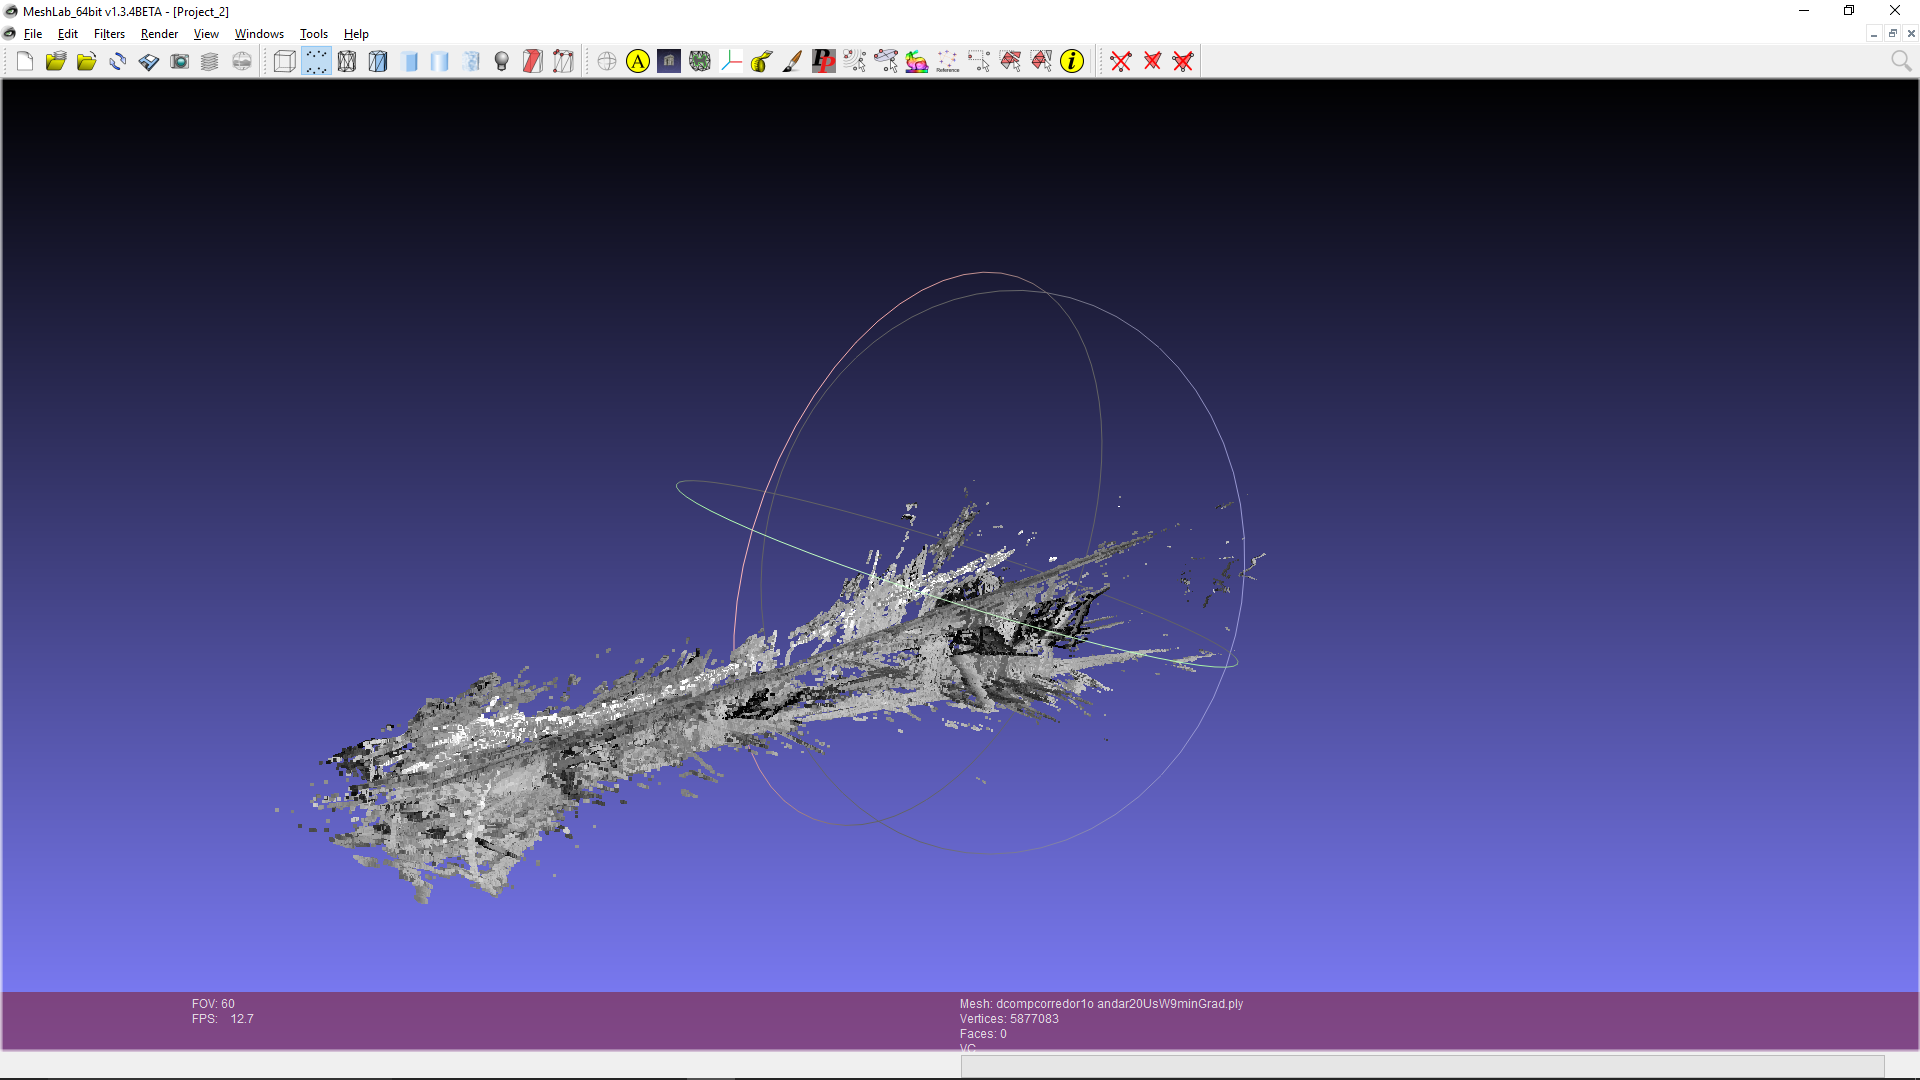
\includegraphics[width= \textwidth]{Imagens/corredorMotox.PNG}
	\caption{\textit{Nuvem de pontos} do corredor do primeiro andar DCOMP usando a câmera do \textit{smartphone Motorola® Moto X Play} com 5877083 pontos}
\end{figure}

\begin{figure}[H]
	\centering
		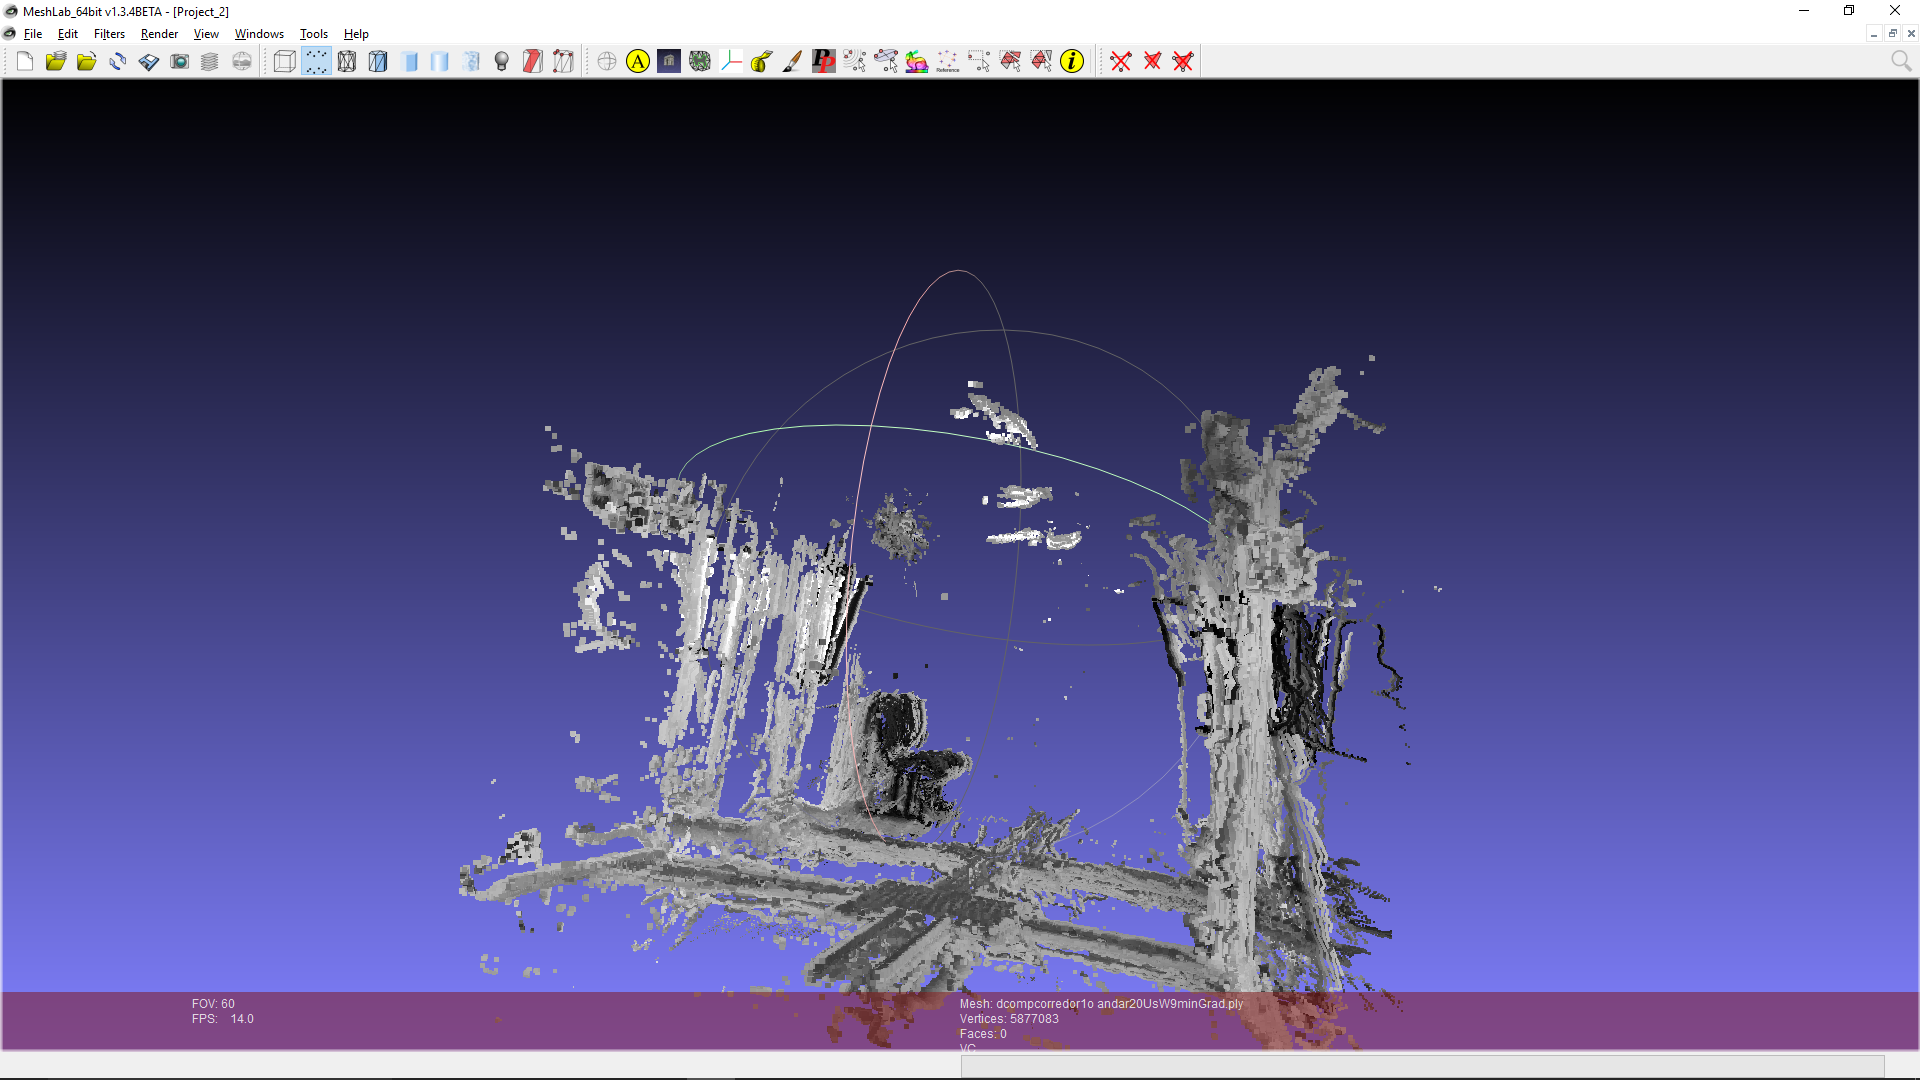
\includegraphics[width= \textwidth]{Imagens/corredorMotoxdentro.PNG}
	\caption{\textit{Nuvem de pontos} do corredor do primeiro andar DCOMP usando a câmera do \textit{smartphone Motorola® Moto X Play} por dentro do \textit{PointCloud} com 5877083 pontos}
\end{figure}

As imagens mostram as saídas do algoritmo em diferentes ambientes. Percebe-se que apesar de haver partes incompletas, os mapas oferecem uma informação correta se usados de maneira adequada. Em algumas dessas imagens percebe-se que a definição de profundidade foi insatisfatória devido ao meio em que foram capturados esses \textit{datasets}, no entanto satisfatória para o intuito original de modelagem 3D proposto na introdução.

\section{Problemas}

Alguns problemas encontrados na gravação do \textit{dataset} foram relacionados à luminosidade. Ela afeta fortemente os quadros capturados fazendo com que as imagens tiradas pela câmera sofram problemas de exposição tornando-os inválidos para processamento. Isso se torna mais evidente em ambientes externos sob forte luminosidade ou ambientes internos com pouca luz. O fato que o algoritmo converte todas as imagens usadas também causa problemas no reconhecimento de gradientes caso duas cores tenham a mesma tonalidade. 

A escolha do equipamento também influencia muito, já que inicialmente foi utilizada uma \textit{webcam} da marca \textit{Logitech®} e frequentemente vários quadros eram encontrados distorcidos, pixelados. Ainda sobre o equipamento, foi notado que a falta de foco também prejudica a reconstrução, dado que o algoritmo não consegue realizar casamentos confiáveis onde um dos quadros está embaçado. As Figuras \ref{fig4:16}, \ref{fig4:17} e \ref{fig4:18}  exemplificam alguns casos onde esses problemas ocorreram. Também houve dificuldade em interligar  \textit{datasets} diferentes para tentar criar uma reconstrução mais completa pois os erros nas transições entre ambientes, como por exemplo de um corredor para uma escada ou de um corredor para outro corredor só são descobertos após o processo de extrair cada quadro do vídeo e rodar o \textit{LSD-SLAM}, fazendo com que seja necessário uma re-captura do \text{dataset}. 

\begin{figure}[H]
	\centering
		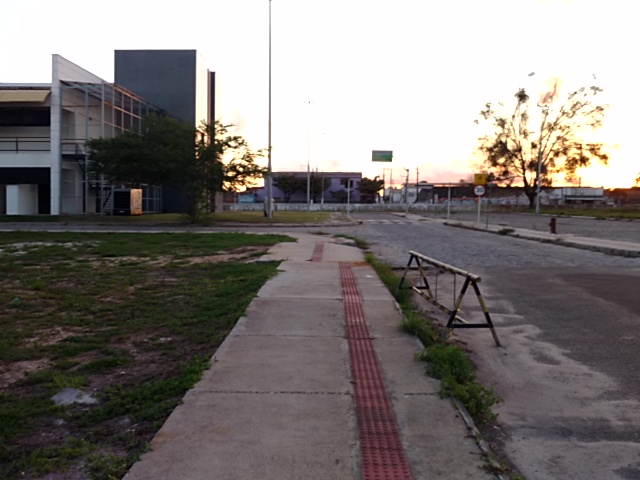
\includegraphics[width= \textwidth]{Imagens/figura4-16.jpg}
		\caption{Fotografia do exterior do prédio do DCOMP, sombras causadas pelo por do sol atrapalham no reconhecimento de gradientes, a reflexividade do prédio faz com um dos lados fique da mesma cor que o céu e a exposição faz com que a imagem tenha saturações}
	\label{fig4:16}
\end{figure}

\begin{figure}[H]
	\centering
		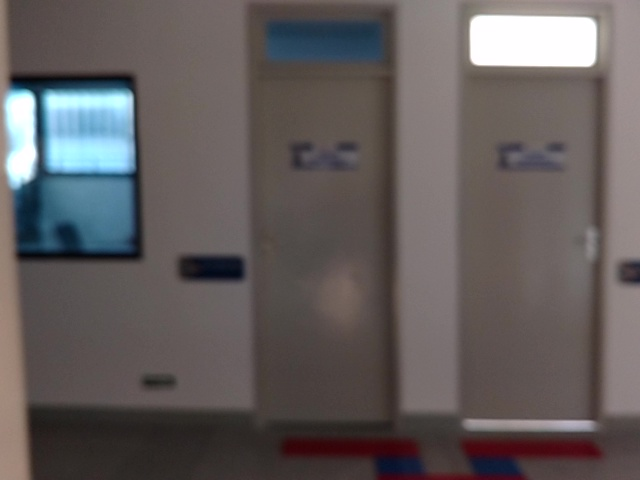
\includegraphics[width= \textwidth]{Imagens/figura4-17.jpg}
	\caption{Fotografia do interior do prédio do DCOMP, desfocado}
	\label{fig4:17}
\end{figure}

\begin{figure}[H]
	\centering
		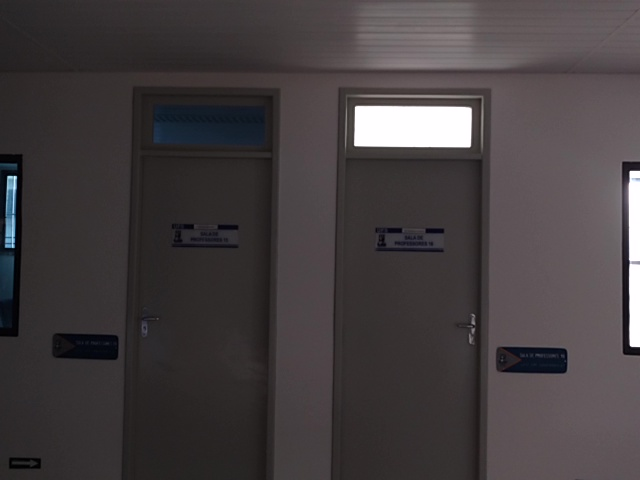
\includegraphics[width= \textwidth]{Imagens/figura4-18.jpg}
	\caption{Fotografia do interior do DCOMP, pouca luminosidade}
	\label{fig4:18}
\end{figure}